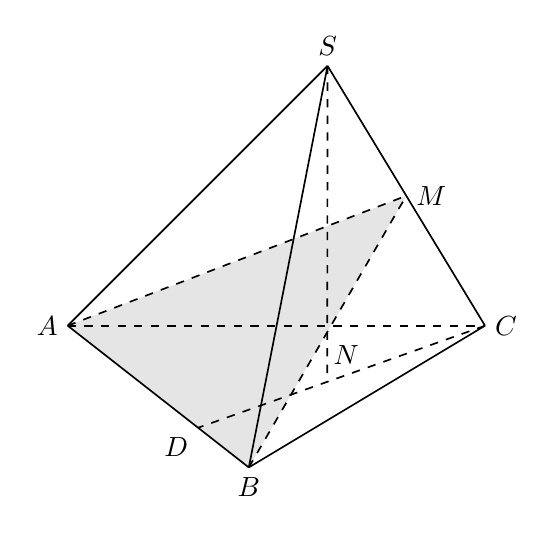
\begin{tikzpicture}[line width=.6pt, font=\normalsize]
  \coordinate (S) at (0.5,3.4);
  \coordinate (A) at (-2.8,0.1);
  \coordinate (C) at (2.5,0.1);
  \coordinate (B) at (-0.5,-1.7);
  \coordinate (N) at (0.4958000000,-0.6128000000);
  \coordinate (D) at (-1.1440000000,-1.1960000000);
  \coordinate (M) at (1.5000000000,1.7500000000);
  % shaded section MAB (gray block, keeps boundary)
  \fill[gray!20] (A) -- (D) -- (B) -- (M) -- cycle;
  % base triangle ABC
  \draw (A) -- (D) -- (B);
  \draw (B) -- (C);
  \draw[dashed] (A) -- (C);
  % lateral edges
  \draw (S) -- (A);
  \draw (S) -- (C);
  \draw (S) -- (B);
  % interior: altitude SN, altitude CD, section edges
  \draw[dashed] (S) -- (N);
  \draw[dashed] (C) -- (D);
  \draw[dashed] (A) -- (M);
  \draw[dashed] (B) -- (M);
  
  \node[above] at (S) {$S$};
  \node[left] at (A) {$A$};
  \node[right] at (C) {$C$};
  \node[below] at (B) {$B$};
  \node[below left] at (D) {$D$};
  \node[right] at (M) {$M$};
  \node[above right=2pt,inner sep=1pt,xshift=-1pt,yshift=3pt] at (N) {$N$};
\end{tikzpicture}
